\documentclass[12pt]{article}
\usepackage{fullpage,graphicx,psfrag,amsmath,amsfonts,verbatim}
\usepackage[small,bf]{caption}
\usepackage{amsthm}
% \usepackage[hidelinks]{hyperref}
\usepackage{hyperref}
\usepackage{bbm} % for the indicator function to look good
\usepackage{color}
\usepackage{mathtools}
\usepackage{fancyhdr} % for the header
\usepackage{booktabs} % for regression table display (toprule, midrule, bottomrule)
\usepackage{adjustbox} % for regression table display
\usepackage{threeparttable} % to use table notes
\usepackage{natbib} % for bibliography
\input newcommand.tex
\bibliographystyle{apalike}
% \setlength{\parindent}{0pt} % remove the automatic indentation

\title{Return to (non) schooling:\\{\large {The potential impact of school holiday reform}}}
\author{Fu Zixuan \\{\small {EMPE research proposal}}}
\date{\today}

\begin{document}
\maketitle
\thispagestyle{empty}
\begin{abstract}
    \noindent  This research proposal applies the marginal treatment effect (MTE) framework to evaluate school holiday reforms. Two commonly discussed reform directions are analyzed: (1) modifying the school calendar by shortening holidays to compensate for reduced school hours during weekdays, and (2) introducing targeted programs to ensure that underserved students benefit from holiday opportunities. Applying the treatment effect literature, this study wants to compare the effectiveness of these two policies against the status quo. The proposal concludes with a discussion on potential data sources and policy implications.
    \bigskip
\end{abstract}

\newpage
\thispagestyle{empty}
\tableofcontents
\newpage

\setcounter{page}{1}

\section{Introduction}

The return to schooling has been studied extensively in economics, representing
a rich strand of literature that combines the empirical results and the
development of novel econometric methods. Well-known examples include
\citet{angrist1991does,imbens1994identification,card2001estimating}. These
studies have not only influenced education policies but have also advanced the
methodological toolkits.

Much attention has been devoted to the returns to schooling, yet in the
meantime the question of non-schooling—school holidays—is almost as old as that
of schooling itself. The appropriate length and structure of school holidays
have long been a subject of debate among policymakers, educators, and
researchers given its different implications for educational outcome and social
equality. For example, summer learning loss has been widely documented in the
education literature \citep{cooper1996effects}.
% This phenomenon refers to the decline in
% academic skills and knowledge that students experience during extended school
% breaks. 
The extent of the loss varies across subjects, grade levels, and socio-economic
groups. Research consistently shows that students from low-income households
are disproportionately affected \citep{morgan2019socio}, as they often lack
access to resources and opportunities that sustain or enhance learning during
the summer, such as summer camps, tutoring programs, or educational travel. As
a result, the academic achievement gap between socio-economic groups often
widens after the holiday, raising equity concerns among policymakers.
Additionally, long holidays can impose significant burdens on working parents,
who may struggle to balance childcare with work obligations. On the other hand,
school holidays are cherished for the opportunities they provide for rest and
leisure, fostering well-being and creativity among students. Indeed, the
cultural and social significance of holidays cannot be overlooked—after all,
who doesn't enjoy a break?

In light of these competing perspectives, one potential approach is to
rearrange the school calendar by shortening the summer break and compensating
for it with a shorter daily in-class schedule throughout the academic year. In
fact, French President Emmanuel Macron made a classical comparison between
France and Germany in terms of school calendar. He argues for a reform that
follows the German system with shorter holiday and longer daily afternoon
off-school activities. A similar reform in the US called year-round schooling
is studied by \citet{mcmullen2012impact}. Others believe that addressing the
education and equality issue requires ensuring all children, particularly those
from low-income families, have access to meaningful vacation experiences,
rather than simply shortening breaks. This is the objective of the "Vacances
apprenantes" program, which was initially introduced as a remedy for learning
losses caused by the pandemic and has since been maintained as an ongoing
initiative.

The proposal aims to evaluate two policies using different methods. The first
policy requires minimal attention to issues associated with treatment effect
estimation due to its mandatory nature. However, the second method applies the
marginal treatment effect (MTE) framework proposed by
\citet{bjorklund1987estimation, heckman2005structural} which is designed to
address issues of selection bias and heterogeneous treatment effects. To
identify the MTE, I consider two potential instrumental variables, one
continuous (distance) and one discrete (cohort enrollment). Since this is an
empirical exercise, I discuss the availability of data and the potential
directions for data collection.\footnote{However, one should not be overly
    optimistic in this regard.} Finally, the proposal concludes with a brief
discussion of the policy implications.

\section{Methodology}
To evaluate the effects of the policies, I assume that students take
standardized tests at two points during the academic year: at the beginning of
the year, with performance denoted as $Y^s$, and at the end of the academic
year (or the start of the summer holiday), with performance denoted as $Y^e$.

The performance measures considered in this evaluation include: (1) academic
scores, and (2) physical and mental health examinations. One hypothesis is that
the policy changes may introduce trade-offs between these dimensions.
Therefore, I take both into considerations.

The two policies differ in several aspects, but the primary distinction in
treatment effect estimation lies in the take-up of the new policy. The first
policy, focused on school calendar reform, is universally applied, whereas the
second policy targets economically disadvantaged children by providing
subsidies or opportunities without requiring mandatory enrollment.

\subsection{Policy 1: school calendar reform}

\paragraph{Treatment and outcome} The treatment in this context is the length of the holiday, denoted by $D$.
Since the number of days in a year is fixed, any reduction in holiday length
will result in a proportional increase in school days. Thus, a specific holiday
length $D = d$ corresponds to a particular school calendar. The potential
outcomes under different school calendars can be expressed as $Y^s(D)$ and
$Y^e(D)$, representing student performance at the start and end of the academic
year, respectively.

While the reform may involve an earlier return to school rather than a later
start to the holiday, without loss of generality, we can adjust the academic
year's span to make these scenarios equivalent. See figure \ref{fig:drawing}
for an illustration.

\begin{figure}
    \centering
    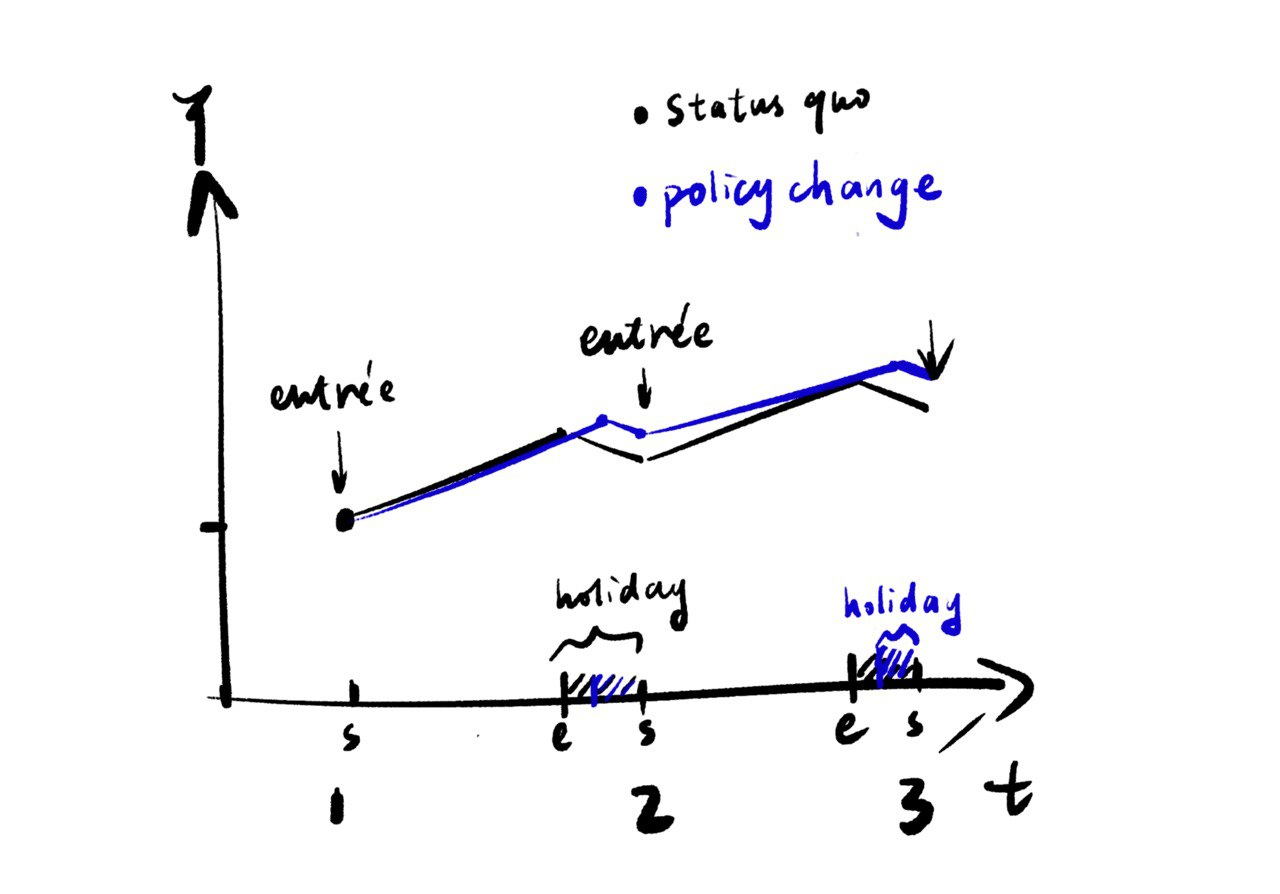
\includegraphics[width=0.5\textwidth]{../Figures/drawing_2.jpg}
    \caption{Illustration of status quo and policy change}
    \label{fig:drawing}
\end{figure}

Previously, I only considered the difference in outcomes before and after the
holiday, expressed as $Y^s_2(D) - Y^e_1(D)$, and compared this difference under
varying holiday lengths. However, this approach provides a narrow look on the
policy reform, as it focuses solely on the holiday period while ignoring its
impact on the regular academic semesters. Naturally, changes to the length of
the holiday will also influence learning during the longer school term, e.g.,
the daily in-school time may be shorter. Therefore, the outcome of interest
should be evaluated from a more holistic perspective, encompassing the entire
academic year, that is $\Delta Y(D)=Y^s_2(D) - Y^s_1(D)$.

\paragraph{Parameter}
The parameter of interest is the Conditional Average Treatment Effect (ATE),
\begin{equation*}
    \text{ATE}(X)=\E\bra{\Delta Y(d')-\Delta Y(d)|X}
\end{equation*}
First, the conditional independence is more likely to hold if we condition on the observed characteristics $X$ (1) socio-economic status and (2) start-of-year performance $Y^s_1$ or the average performance in the previous years. Second, it is of empirical interests to condition on $X$ to examine the
differential impact of the policy on various population groups. This allows for
an analysis of potential equity concerns. Since this policy is mandatory across
all French schools, issues related to selection into treatment can be safely
ignored.

\subsection{Policy 2: learning holiday programs}
\paragraph{Treatment, outcome and selection}
I simplify the change introduced by the second policy as a binary enrollment
treatment, denoted by $D$. Under this policy, the school calendar remains
unchanged, meaning the only source of variation arises from participation in
the new programs. However, for comparability with the first policy, we still
define the potential outcome variable as $\Delta Y(D) = Y^s_2(D) - Y^s_1(D)$.

The learning holiday program\footnote{For further details, consult
    \url{https://www.education.gouv.fr/les-vacances-apprenantes-303834}.} targets a
subpopulation, primarily students in precarious socio-economic situations or
from rural areas. As is common with such targeted programs, there is a
self-selection issue that can either attenuate or amplify the estimated
treatment effect. To address this, I rely on the marginal treatment effect
(MTE) framework \citep{heckman2005structural} to account for selection bias.

The potential outcome of attending the program is modeled as:
\begin{equation*}
    \Delta Y(1)=\mu_1(X)+U_1
\end{equation*} where $X$ represents observed covariates, including (1)
socio-economic characteristics such as household income and (2) baseline performance $Y^s_1$, or the average score from previous
years. $U_1$ represents unobserved factors affecting the outcome.

The choice to participate in the program is determined by the following
equation:
\begin{equation*}
    D=\1\set{\mu_D(X,Z)-U_D\ge 0 }
\end{equation*}
where $X$ is the same set of covariates as in the potential outcome equation, and $Z$ is an additional instrumental variable that is crucial for identifying the marginal treatment effect. Two natural candidates for $Z$ are (1) The distance between the student's home and the program location.
(2) The number of participants (take-up rate) from the student's class (peer effect).

\paragraph{Treatment effect}
The parameter of interest is again the conditional average treatment effect
(ATE). To estimate the ATE, the marginal treatment effect (MTE) is first
estimated, and the ATE is then obtained as a weighted (weight $h = 1$ for the
ATE) sum of the MTE. Given the importance of MTE, I review the local
instrumental variable (LIV) approach in estimating the MTE $\Delta^{\text{MTE}}
    (x,u)$.

Recall the choice equation $D=\1\set{\mu(X,Z)\ge U_D}$, which is equivalent to
$$D=\1\set{F_{U_D}(\mu(X,Z))\ge F_{U_D}(U_D)}= \1\set{\tilde{\mu}(X,Z)\ge
        \tilde{U}_D}$$ with $\tilde{U}_D\sim U[0,1]$. Therefore, it is without loss of
generality to assume $U_D\sim U[0,1]$. Thus
\begin{equation}
    \mu(X,Z)=\p(D=1|X,Z)
\end{equation}
The essence of LIV is this equality. Since we do not directly observe the $U_D$, we can not directly get $\E[Y|X=x,U_D=u]$. However, we can directly observe $\p(D=1|X=x,Z=z)$ and therefore $\E[Y|X=x,P(D=1|X=x,Z=z)=p]$. \citet{heckman2005structural} shows that
\begin{equation*}
    \E[Y|X=x,U_D=p]=\frac{\partial \E[Y|X=x,P(D=1|X=x,Z=z)=p]}{\partial p}
\end{equation*}
In order to get the standard treatment effect parameter $\text{ATE}(x)$, we need \begin{itemize}
    \item $P(D=1|X=x,Z)$ has the full support on $(0,1)$.
    \item $\p(D=1|X=x,Z)$ is continuous so as to take the derivative.
    \item a polynomial MTE model if the local instrument is discrete
          \citep{brinch2017beyond}.
\end{itemize}
\paragraph{The first candidate} $Z_1$--distance--gives a continuous local
instrument $\p(D=1|X=x,Z)$. I intend to use a nonparametric approach to
directly estimate the derivative function since I do not include too many
covariates. \paragraph{The second candidate} $Z_2$--the number of classmates enrolled--is an
instrument that deserves a closer examination. Recall some of the assumptions
maintained in the analysis are:
\begin{enumerate}
    \item $\mu_D(Z)$ is a nondegenerate random variable conditional on $X$.
    \item $(U_1, U_D)$ and $(U_0, U_D)$ are independent of $Z$ conditional on $X$.
    \item $1 > P(D=1|Z) > 0$.
\end{enumerate}
First, it is reasonable to assume that other's enrollment affect my decision and assumption 1 and 3 are likely to hold. Second, even though my decision $D=\1\set{\mu_D(X,Z)-U_D\ge 0}$ affects the number of participants $Z_2$ by peer effect, it should be negligible since the class size is not too small. In this case, I may assume that assumption 2 holds. Lastly, since if $Z_2$ takes on $N$ values, a polynomial of order $L\le N$ MTE model is to be specified and identified as in \citet{brinch2017beyond}.
\section{Discussion}
\subsection{Data}
One potential source is the OECDs Programme for International Student
Assessment (PISA), a project that evaluates the education systems of countries
around the world by testing the skills and knowledge of 15-year-old students.
PISA provides information on student performance in mathematics, reading, and
science, along with data on socio-economic background and school
characteristics.

Ideally, it would be best to collect not only academic data but also physical
and mental health data of students at both the beginning and the end of the
academic year. For the learning holiday initiative, the current information is
limited to anecdotal evidence from news reports and participant feedback since
its launch in 2020. As the program is relatively new, more data needs to be
collected to evaluate its quantitative impact comprehensively.

In addition to the performance outcomes $Y$ and student characteristics $X$
mentioned earlier, other relevant information, such as the distance between the
student's home and the program location, as well as the number of participants
from the same class, is essential for dealing with selection on unobservables.
However, the data collection plan described above represents an ideal scenario
that may not be fully attainable in practice.\footnote{Sometimes in a research
    proposal, one can dream big and bold.}

\subsection{Pilot study}
Since different countries and regions operate under varying school calendars,
there are natural control and treatment groups available for analysis. However,
this is not exactly what I originally intended. The PISA surveys test different
cohorts of students triennially, rather than following the same cohort over
time. At a pilot or exploratory stage, it may be of interest to adopt the
following standard approaches:

\begin{itemize}
    \item Regard students from different countries as directly comparable when
          conditioned on a set of individual and school characteristics. The treatment
          effect of holiday length can be estimated by regressing performance on holiday
          length and other covariates.
    \item If there is a policy change in some countries but not in others, a
          difference-in-differences (DiD) heterogeneous two-way fixed effects model
          \citet{de2023two} can be employed to estimate the effect of holiday length,
          $d$.
\end{itemize}
% \footnote{Though the results are not likely to be
%     reliable, it is a starting point to test the methods and identify potential
%     issues.}
\pagebreak
\newpage
\bibliography{ref.bib}

\end{document}